\section{Computational experiments}
\label{computational_experiments}
This section evaluates the proposed algorithm on real data from five Spanish cities with different urban characteristics. We first describe the data and the experimental design. We then compare the survival strategies of NSGA-II and NSGA-III and the three- and four-objective formulations, study whether recombination helps, assess the contribution of each component of the algorithm, examine the equity measure, bound the accessibility of the solutions, and finally compare them with the layouts currently deployed in each city.

\subsection{Data preparation}
For each city, the candidate locations for UCO containers are the sites of the other container types (organic waste, paper, plastic, etc.) available in the municipal open data portals\footnote{Portals used: \url{https://valencia.opendatasoft.com}, \url{https://www.donostia.eus/datosabiertos/}, \url{https://opendata.esri.es/datasets/ideSEVILLA::contenedores-de-recogida-de-residuos/}, \url{https://datosabiertos.malaga.eu/}, \url{https://www10.ava.es/portalva/apps/webappviewer/index.html?id=40aa1fa90bfa43578280d3943779e273}}. These sites already have accessibility, municipal permits and maintenance, which minimizes implementation barriers. Since many of them are clustered within short distances, candidates closer than 50\,m to another one are removed. The sites of the existing UCO containers are added to the candidates, so the current layout belongs to the search space. Population comes from GHS-POP R2023A (epoch 2030 for Donostia, Valladolid and Valencia, 2025 for Málaga and Sevilla). Table~\ref{city_summary} summarizes the five instances.

\begin{table}[htbp]
\caption{The five instances: candidate locations (after the 50\,m filter), current UCO containers, population in the study area, area, density, current inhabitants per container, and share of the population that the current network can serve with $\alpha = 1000$.}
\centering
\small
\label{city_summary}
\begin{tabular}{lrrrrrrr}
\toprule
\textbf{City} & \textbf{Candidates} & \textbf{Current} & \textbf{Population} & \textbf{Area (km\textsuperscript{2})} & \textbf{Density (inh./km\textsuperscript{2})} & \textbf{Inh./container} & \textbf{Capacity share} \\
\midrule
Donostia   & 674  & 111 & 179,963 & 18.9 & 9,506  & 1,621 & 62\% \\
Valladolid & 1,235 & 174 & 273,403 & 39.0 & 7,006  & 1,571 & 64\% \\
Valencia   & 3,234 & 352 & 796,497 & 61.6 & 12,936 & 2,263 & 44\% \\
Málaga     & 1,842 & 90  & 528,324 & 66.0 & 8,004  & 5,870 & 17\% \\
Sevilla    & 1,744 & 96  & 687,205 & 69.9 & 9,833  & 7,158 & 14\% \\
\bottomrule
\end{tabular}
\end{table}

The service level $\alpha$ is defined from container capacity and waste generation. UCO containers typically have a capacity of 450 liters, while the estimated amount of waste cooking oil generated per person per year is 4 liters according to Spanish environmental authorities \cite{miteco}. Approximately 11 liters of UCO are therefore generated per day for every 1,000 inhabitants and, if all of it were collected, a container would be full in about 41 days, in line with monthly to bi-monthly municipal collection cycles. Accordingly, we set $\alpha = 1000$ inhabitants per container. As the last column of Table~\ref{city_summary} shows, no city has enough containers to serve its whole population at this level, and Málaga and Sevilla are far from it.

\subsection{Experimental setup}
For each city, the range of network sizes is from half to 1.5 times the current number of containers, $k_{\min} = \lfloor k_0/2 \rfloor$ and $k_{\max} = \mathrm{round}(1.5\, k_0)$, divided into $m = 11$ allowed sizes plus $k_0$. Every run lasts $G = 300$ generations with a population of $\mu = 100$, mutation probability $p_m = 0.5$, moved share $\beta = 0.02$, local-move probability $p_\ell = 0.8$ and resize probability $p_r = 0.2$; when a crossover is used, its probability is $p_c = 0.9$. These values were set by hand on Donostia and kept for all cities and variants.

We report five studies, all with 30 independent runs per variant and city, each run on one dedicated core of a computing cluster:
\begin{enumerate}
\item a full factorial design with the survival strategy (NSGA-II or NSGA-III), the formulation (three objectives, $f_1$--$f_3$, or four, $f_1$--$f_4$) and the crossover (regional with large regions, $\rho \in [0.1, 0.5]$, or uniform);
\item a study of recombination with NSGA-II and four objectives: no crossover, and regional and graph crossover with parameters tuned beforehand (Section~\ref{sec:recombination});
\item an ablation of the recommended configuration (NSGA-II, four objectives, no crossover), removing one component at a time;
\item the robustness of the equity measure to its parameters and its relation to classical measures;
\item lower bounds on the accessibility that can be reached with today's number of containers.
\end{enumerate}
In total, the studies comprise 3,490 runs (including the tuning runs), plus 5 runs per city of the single-objective algorithm of the deployed service for comparison. A run without crossover took between 15\,s (Donostia) and 38\,s (Sevilla); with crossover, between 25\,s and 118\,s (Section~\ref{sec:recombination}).

The quality of a front is measured by its hypervolume (HV) \cite{zitzler1999multiobjective}. For each city, the objectives are normalized to $[0,1]$ with bounds common to all the variants of studies 1 and 2: $f_1$ over $[k_{\min}, k_{\max}]$, $f_2$ and $f_4$ between the best and worst values found (or the value of the current layout, if worse), and $f_3$ between 0 and the worst value. The reference point is $1.1$ in every objective. Each variant is scored in the space of its own formulation (HV3 or HV4); since every run records the four objectives of its layouts, the formulations are also compared by scoring all fronts in both spaces. Variants are compared per city with the two-sided Mann--Whitney U test, with Holm's correction for all the comparisons made in each city, and with the Vargha--Delaney $\hat{A}_{12}$ effect size \cite{vargha2000critique}, the probability that a run of one variant beats a run of the other.

\subsection{Survival strategy and formulation}
\begin{table}[htbp]
\centering
\small
\caption{Hypervolume after 300 generations, mean (standard deviation) of 30 runs, in the objective space of each formulation (HV3 or HV4); the best of each row in bold. $\hat{A}_{12}$: Vargha--Delaney effect size, the probability that a run of the first variant beats a run of the second, for regional (RX) against uniform (UX) crossover and for NSGA-III against NSGA-II (both with RX). Mann--Whitney U tests with Holm correction within each city; $^\dagger$: not significant at $\alpha = 0.05$.}
\label{tab:hv}
\resizebox{\textwidth}{!}{%
\begin{tabular}{llccccccc}
\toprule
& & \multicolumn{2}{c}{\textbf{NSGA-II}} & \multicolumn{2}{c}{\textbf{NSGA-III}} & \multicolumn{3}{c}{$\hat{A}_{12}$} \\
\cmidrule(lr){3-4} \cmidrule(lr){5-6} \cmidrule(lr){7-9}
\textbf{City} & \textbf{Obj.} & RX & UX & RX & UX & RX/UX (II) & RX/UX (III) & III/II \\
\midrule
\multirow{2}{*}{Donostia} & 3 & \textbf{0.6819 (0.0041)} & 0.6619 (0.0054) & 0.6802 (0.0050) & 0.6597 (0.0036) & 1.00 & 1.00 & 0.39$^\dagger$ \\
 & 4 & 0.6302 (0.0063) & 0.6042 (0.0089) & \textbf{0.6303 (0.0066)} & 0.5991 (0.0079) & 1.00 & 1.00 & 0.51$^\dagger$ \\
\midrule
\multirow{2}{*}{Valladolid} & 3 & \textbf{0.5831 (0.0058)} & 0.5735 (0.0061) & 0.5762 (0.0076) & 0.5629 (0.0067) & 0.87 & 0.91 & 0.23 \\
 & 4 & \textbf{0.5147 (0.0049)} & 0.4880 (0.0061) & 0.5130 (0.0057) & 0.4839 (0.0074) & 1.00 & 1.00 & 0.40$^\dagger$ \\
\midrule
\multirow{2}{*}{Valencia} & 3 & \textbf{0.5888 (0.0061)} & 0.5752 (0.0057) & 0.5840 (0.0070) & 0.5720 (0.0070) & 0.96 & 0.89 & 0.29 \\
 & 4 & 0.5309 (0.0079) & 0.5005 (0.0131) & \textbf{0.5318 (0.0069)} & 0.4972 (0.0109) & 0.97 & 1.00 & 0.52$^\dagger$ \\
\midrule
\multirow{2}{*}{Málaga} & 3 & \textbf{0.6352 (0.0045)} & 0.6154 (0.0053) & 0.6344 (0.0054) & 0.6167 (0.0055) & 1.00 & 0.99 & 0.44$^\dagger$ \\
 & 4 & \textbf{0.6160 (0.0048)} & 0.5853 (0.0069) & 0.6160 (0.0037) & 0.5858 (0.0079) & 1.00 & 1.00 & 0.51$^\dagger$ \\
\midrule
\multirow{2}{*}{Sevilla} & 3 & 0.6525 (0.0038) & 0.6392 (0.0036) & \textbf{0.6528 (0.0029)} & 0.6378 (0.0037) & 1.00 & 1.00 & 0.54$^\dagger$ \\
 & 4 & \textbf{0.6345 (0.0058)} & 0.6076 (0.0074) & 0.6322 (0.0069) & 0.6010 (0.0080) & 1.00 & 1.00 & 0.37$^\dagger$ \\
\bottomrule
\end{tabular}}
\end{table}


\begin{figure}[htbp]
    \centering
    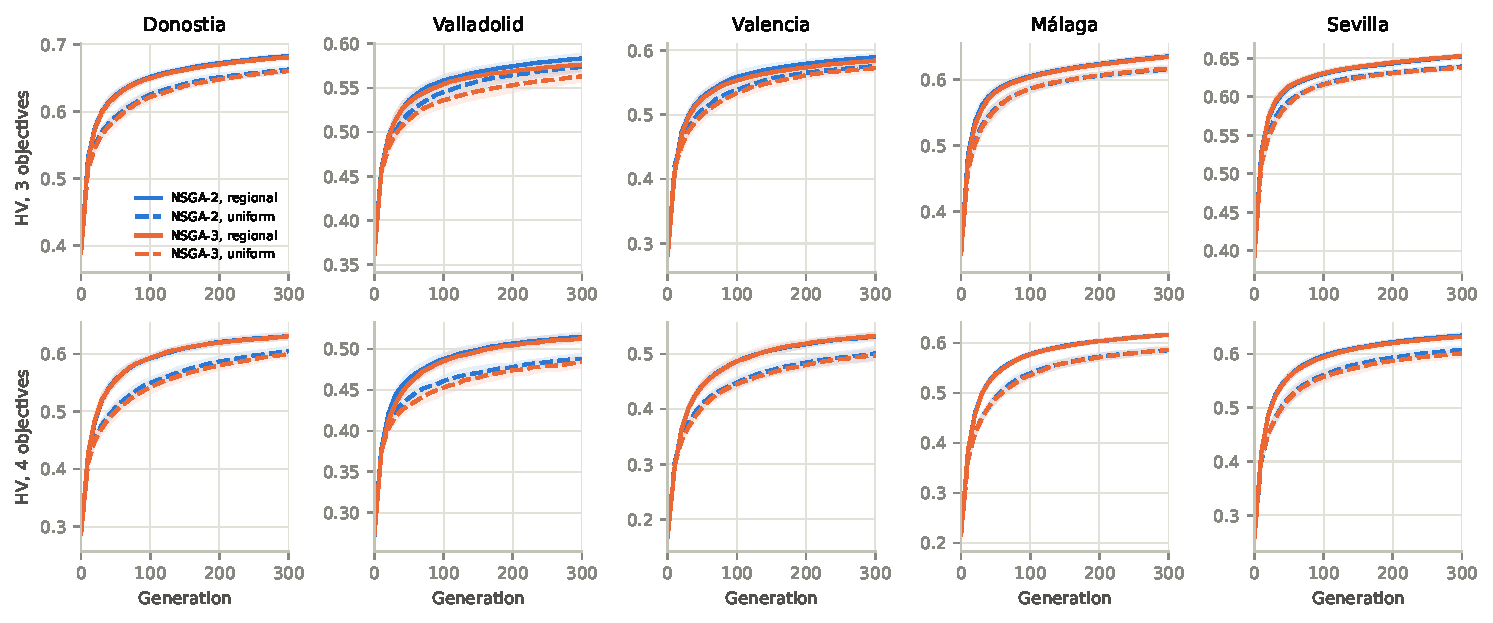
\includegraphics[width=\textwidth]{figures/convergence.pdf}
    \caption{Hypervolume of the front along the generations in the factorial study, in the space of each formulation: mean and standard deviation of 30 runs per variant. Colour: survival strategy; line style: crossover.}
    \label{fig:convergence}
\end{figure}

Table~\ref{tab:hv} and Figure~\ref{fig:convergence} show the factorial study. NSGA-III, designed for problems with many objectives, brings no improvement (last column). With three objectives, the differences are not significant in three cities, and NSGA-II is significantly better in Valladolid ($\hat{A}_{12} = 0.23$ for NSGA-III) and Valencia ($0.29$); with four objectives, no difference is significant ($0.37 \leq \hat{A}_{12} \leq 0.52$). We attribute this to the structure of the problem: the discrete set of sizes already spreads the population along $f_1$, and the guided mutation, rather than the survival step, drives the search (Section~\ref{sec:ablation}). Since NSGA-II is simpler and needs no reference directions, we use it in the rest of the paper and in the service. The two crossovers of this study are compared in Section~\ref{sec:recombination}.

\begin{table}[htbp]
\centering
\small
\caption{The fronts of both formulations (NSGA-II without crossover) scored in both objective spaces: HV3 (containers, unserved people, inequity) and HV4 (plus mean distance), mean (standard deviation) of 30 runs, with the Vargha--Delaney $\hat{A}_{12}$ of the four-objective against the three-objective formulation (Holm-corrected Mann--Whitney U; $^\dagger$: not significant).}
\label{tab:formulation}
\begin{tabular}{lcccccc}
\toprule
& \multicolumn{3}{c}{\textbf{HV3}} & \multicolumn{3}{c}{\textbf{HV4}} \\
\cmidrule(lr){2-4} \cmidrule(lr){5-7}
\textbf{City} & 3 obj. & 4 obj. & $\hat{A}_{12}$ & 3 obj. & 4 obj. & $\hat{A}_{12}$ \\
\midrule
Donostia & 0.7082 (0.0026) & 0.6893 (0.0035) & 0.00 & 0.6194 (0.0101) & 0.6554 (0.0051) & 1.00 \\
Valladolid & 0.6009 (0.0096) & 0.5848 (0.0075) & 0.07 & 0.4766 (0.0194) & 0.5248 (0.0077) & 1.00 \\
Valencia & 0.6143 (0.0060) & 0.6014 (0.0046) & 0.04 & 0.5155 (0.0118) & 0.5480 (0.0078) & 0.99 \\
Málaga & 0.6637 (0.0052) & 0.6420 (0.0034) & 0.00 & 0.5334 (0.0176) & 0.6308 (0.0039) & 1.00 \\
Sevilla & 0.6745 (0.0036) & 0.6581 (0.0025) & 0.00 & 0.5240 (0.0184) & 0.6423 (0.0053) & 1.00 \\
\bottomrule
\end{tabular}
\end{table}


Table~\ref{tab:formulation} scores the fronts of both formulations (NSGA-II without crossover) in both objective spaces. Adding distance as a fourth objective has a small cost in the three-objective space, where the HV3 of the four-objective fronts is between 2.1\% (Valencia) and 3.3\% (Málaga) lower, and a large gain in the four-objective space, where their HV4 is between 5.8\% (Donostia) and 22.6\% (Sevilla) higher. Both differences are significant in every city. The same holds with regional crossover and with NSGA-III.

\begin{figure}[htbp]
    \centering
    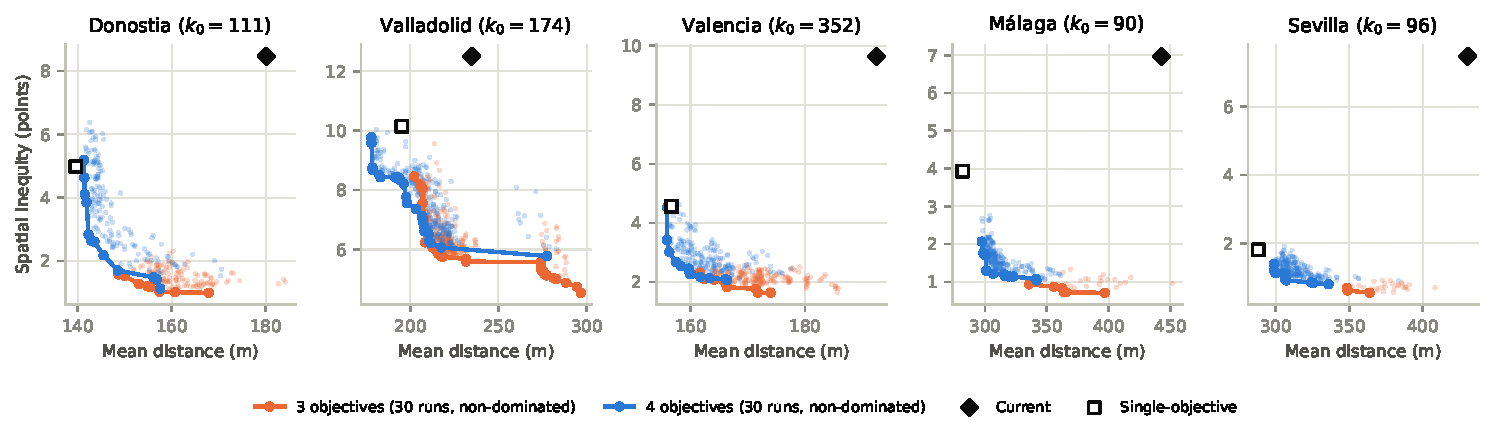
\includegraphics[width=\textwidth]{figures/tradeoff_k0.pdf}
    \caption{Layouts with today's number of containers $k_0$ and no more unserved people than today, from the 30 fronts of each formulation (NSGA-II without crossover), in the plane of mean distance and spatial inequity; lines join the non-dominated ones. Diamond: current layout; square: single-objective algorithm (median of 5 runs).}
    \label{fig:tradeoff}
\end{figure}

Figure~\ref{fig:tradeoff} shows what this means for a planner who keeps today's number of containers. The three-objective fronts concentrate on the fairest layouts and leave accessibility to chance: in Málaga and Sevilla their layouts are 330--400\,m away on average, 50--115\,m more than the single-objective solution. The four-objective fronts cover the whole trade-off, from layouts as accessible as the single-objective solution, and fairer, to layouts nearly as fair as the three-objective ones. In Valladolid and Valencia they include layouts that dominate the single-objective solution in both distance and inequity; in Donostia, Málaga and Sevilla, layouts within 2--15\,m of its distance with less inequity.

\subsection{Recombination}
\label{sec:recombination}
The factorial study shows a large and consistent advantage of the regional crossover over the uniform crossover (Table~\ref{tab:hv}): it wins in all 20 comparisons, with $\hat{A}_{12} \geq 0.87$. This does not mean that recombination helps, only that one crossover is less harmful than the other. To find out, we compared crossovers with no crossover at all, after giving each spatial crossover a fair chance. Both were tuned with the same protocol on two cities (Donostia and Valencia, 10 runs each): the regional crossover over six ranges of region size, from $\rho \in [0.001, 0.005]$ to $[0.1, 0.5]$, and the graph crossover over ten combinations of the number of subgraphs $g \in \{1, 3, 10\}$ and their depth $h \in \{1, \dots, 20\}$. The configuration with the best mean rank over both cities was kept: the smallest regions for the regional crossover ($[0.001, 0.005]$, i.e., 1--16 candidates), and one subgraph of depth 1 (a candidate and its Delaunay neighbours) for the graph crossover. In both cases, the smaller the exchanged region, the better.

\begin{table}[htbp]
\centering
\small
\caption{Recombination (NSGA-II, four objectives): HV4 after 300 generations, mean (standard deviation) of 30 runs, without crossover and with four crossovers: regional and graph crossover with small regions (tuned, Section~\ref{sec:recombination}), regional crossover with large regions (10--50\% of the candidates) and uniform crossover. $\hat{A}_{12}$: probability that a run with the crossover beats a run without it (Holm-corrected Mann--Whitney U; $^\dagger$: not significant).}
\label{tab:recombination}
\resizebox{\textwidth}{!}{%
\begin{tabular}{lccccccccc}
\toprule
& \textbf{None} & \multicolumn{2}{c}{\textbf{Regional, small}} & \multicolumn{2}{c}{\textbf{Graph, small}} & \multicolumn{2}{c}{\textbf{Regional, large}} & \multicolumn{2}{c}{\textbf{Uniform}} \\
\cmidrule(lr){3-4} \cmidrule(lr){5-6} \cmidrule(lr){7-8} \cmidrule(lr){9-10}
\textbf{City} & HV4 & HV4 & $\hat{A}_{12}$ & HV4 & $\hat{A}_{12}$ & HV4 & $\hat{A}_{12}$ & HV4 & $\hat{A}_{12}$ \\
\midrule
Donostia & 0.6554 (0.0051) & 0.6528 (0.0044) & 0.31 & 0.6507 (0.0053) & 0.25 & 0.6302 (0.0063) & 0.00 & 0.6042 (0.0089) & 0.00 \\
Valladolid & 0.5248 (0.0077) & 0.5209 (0.0074) & 0.37$^\dagger$ & 0.5221 (0.0057) & 0.40$^\dagger$ & 0.5147 (0.0049) & 0.13 & 0.4880 (0.0061) & 0.00 \\
Valencia & 0.5480 (0.0078) & 0.5506 (0.0076) & 0.58$^\dagger$ & 0.5490 (0.0104) & 0.54$^\dagger$ & 0.5309 (0.0079) & 0.06 & 0.5005 (0.0131) & 0.00 \\
Málaga & 0.6308 (0.0039) & 0.6316 (0.0047) & 0.58$^\dagger$ & 0.6305 (0.0041) & 0.50$^\dagger$ & 0.6160 (0.0048) & 0.01 & 0.5853 (0.0069) & 0.00 \\
Sevilla & 0.6423 (0.0053) & 0.6446 (0.0053) & 0.63$^\dagger$ & 0.6447 (0.0053) & 0.61$^\dagger$ & 0.6345 (0.0058) & 0.18 & 0.6076 (0.0074) & 0.00 \\
\bottomrule
\end{tabular}}
\end{table}


Table~\ref{tab:recombination} shows the result. Recombination brings no improvement. The tuned crossovers are statistically indistinguishable from no crossover in four cities, and worse in Donostia ($\hat{A}_{12} = 0.31$ and $0.25$); the crossovers with large regions and the uniform crossover are clearly worse in every city ($\hat{A}_{12} \leq 0.18$). Moreover, the best crossovers exchange so few locations that they act as an additional mutation. No crossover is also cheaper: since half of the offspring are unmutated copies of their parents, which need no new evaluation, a run is 1.6 to 2.4 times faster than with the small-region crossovers, and up to three times faster than with the large ones. We therefore recommend, and use in the service, NSGA-II without crossover. In our problem, the locations interact through the Voronoi cells and the shares of their neighbourhoods; exchanging even small, spatially coherent parts between two good layouts breaks those interactions more often than it combines their strengths, while small guided moves improve them.

\subsection{Ablation}
\label{sec:ablation}
\begin{table}[htbp]
\centering
\small
\caption{Ablation of the recommended configuration (NSGA-II, four objectives, no crossover): HV4, mean of 30 runs, with one component removed at a time: the discrete set of sizes (all sizes in the range allowed), the load-guided resizing (random instead), the comparison of $f_2$ in steps (exact values), the local moves of the mutation (all moves to random candidates) and the seeding of the current layout. $\hat{A}_{12}$: probability that a run of the full configuration beats a run without the component (Holm-corrected Mann--Whitney U; $^\dagger$: not significant).}
\label{tab:ablation}
\resizebox{\textwidth}{!}{%
\begin{tabular}{lccccccccccc}
\toprule
& \textbf{Full} & \multicolumn{2}{c}{\textbf{All sizes}} & \multicolumn{2}{c}{\textbf{Random resize}} & \multicolumn{2}{c}{\textbf{Exact $f_2$}} & \multicolumn{2}{c}{\textbf{No local moves}} & \multicolumn{2}{c}{\textbf{No seed}} \\
\textbf{City} & HV4 & HV4 & $\hat{A}_{12}$ & HV4 & $\hat{A}_{12}$ & HV4 & $\hat{A}_{12}$ & HV4 & $\hat{A}_{12}$ & HV4 & $\hat{A}_{12}$ \\
\midrule
Donostia & 0.6554 & 0.5170 & 1.00 & 0.4960 & 1.00 & 0.6465 & 0.84 & 0.6349 & 0.99 & 0.6557 & 0.52$^\dagger$ \\
Valladolid & 0.5248 & 0.3962 & 1.00 & 0.4103 & 1.00 & 0.5183 & 0.72 & 0.5128 & 0.88 & 0.5232 & 0.56$^\dagger$ \\
Valencia & 0.5480 & 0.3011 & 1.00 & 0.3292 & 1.00 & 0.5382 & 0.82 & 0.5251 & 0.96 & 0.5491 & 0.46$^\dagger$ \\
Málaga & 0.6308 & 0.5167 & 1.00 & 0.4955 & 1.00 & 0.6041 & 0.99 & 0.6050 & 1.00 & 0.6292 & 0.61$^\dagger$ \\
Sevilla & 0.6423 & 0.5284 & 1.00 & 0.5262 & 1.00 & 0.6257 & 0.97 & 0.6238 & 1.00 & 0.6458 & 0.31 \\
\bottomrule
\end{tabular}}
\end{table}


Table~\ref{tab:ablation} removes one component of the recommended configuration at a time. The discrete set of sizes and the load-guided resizing are essential: without either of them, the HV4 drops by 18--45\% in every city ($\hat{A}_{12} = 1.00$). Allowing all sizes spreads the population too thinly for layouts of the same size to compete, and random resizing adds and removes containers where they matter least. The local moves of the mutation and the comparison of $f_2$ in steps of 100 people also contribute significantly in every city ($0.72 \leq \hat{A}_{12} \leq 1.00$). Seeding the current layout makes no difference in four cities, and in Sevilla it is slightly worse ($\hat{A}_{12} = 0.31$); its purpose is to guarantee that the front is never worse than the existing deployment, not to speed up the search.

\subsection{The equity measure}
\label{sec:equity_results}
\begin{table}[htbp]
\centering
\small
\caption{Spearman rank correlation between $f_3$ (500\,m blocks, 1\,km neighbourhoods) and other measures, over the layouts with today's number of containers of the 30 fronts of each city (NSGA-II, four objectives, no crossover): $f_3$ with other block sizes and radii, Moran's I of the blocks, and classical non-spatial measures \cite{marsh1994equity}: population-weighted Gini coefficients of the unserved share of each person, of the load of each container and of the distance to the nearest container.}
\label{tab:equity}
\resizebox{\textwidth}{!}{%
\begin{tabular}{lrccccccc}
\toprule
\textbf{City} & \textbf{Layouts} & $f_3$ 250/500 & $f_3$ 1000/2000 & Moran's I & Gini unserved & Gini load & Gini distance & Mean distance \\
\midrule
Donostia & 171 & +0.88 & +0.90 & +0.85 & +0.06 & -0.37 & -0.73 & -0.80 \\
Valladolid & 318 & +0.86 & +0.83 & +0.66 & +0.25 & -0.57 & -0.54 & -0.84 \\
Valencia & 192 & +0.65 & +0.86 & +0.75 & -0.31 & -0.41 & -0.20 & -0.62 \\
Málaga & 237 & +0.80 & +0.90 & +0.75 & +0.29 & +0.27 & -0.51 & -0.81 \\
Sevilla & 212 & +0.72 & +0.83 & +0.68 & +0.21 & +0.21 & -0.41 & -0.65 \\
\bottomrule
\end{tabular}}
\end{table}


Table~\ref{tab:equity} correlates $f_3$ with other measures over the layouts with today's number of containers of the 30 fronts of each city. $f_3$ is robust to its parameters: with blocks of 250\,m and neighbourhoods of 500\,m, or with blocks of 1\,km and neighbourhoods of 2\,km, it ranks the layouts in a similar order (Spearman $\rho$ between 0.65 and 0.90). The comparison of crossovers does not depend on these parameters either (Table~\ref{tab:sensitivity}): the regional crossover beats the uniform crossover in every city with both alternative settings ($\hat{A}_{12} \geq 0.96$). Moran's I of the blocks, computed on the same fixed support, is also correlated with $f_3$ ($0.66 \leq \rho \leq 0.85$): the intuition of the earlier formulation was sound, its shortcomings were the changing support and the insensitivity to magnitude. Conversely, the classical non-spatial measures rank the layouts differently: the Gini coefficient of the unserved share of each person is almost unrelated to $f_3$ ($-0.31 \leq \rho \leq 0.29$), and the Gini coefficient of the loads is weakly and inconsistently related to it ($-0.57 \leq \rho \leq 0.27$). They measure how unequal the shortage is, not where it is. Finally, $f_3$ is negatively correlated with the mean distance ($-0.62 \leq \rho \leq -0.84$) and with the Gini coefficient of distances: fairer layouts spread containers towards less dense areas, which lengthens the average walk, the trade-off that motivates $f_4$.

\begin{table}[htbp]
\centering
\small
\caption{Sensitivity of the comparison between regional (large regions) and uniform crossover to the parameters of $f_3$ (NSGA-II, four objectives, 30 runs): HV4 with blocks of 250\,m and neighbourhoods of 500\,m, and with blocks of 1\,km and neighbourhoods of 2\,km (each normalized among its own runs), and $\hat{A}_{12}$ of regional against uniform (all differences significant, $p < 10^{-9}$).}
\label{tab:sensitivity}
\begin{tabular}{lcccccc}
\toprule
& \multicolumn{3}{c}{\textbf{250\,m / 500\,m}} & \multicolumn{3}{c}{\textbf{1\,km / 2\,km}} \\
\cmidrule(lr){2-4} \cmidrule(lr){5-7}
\textbf{City} & Regional & Uniform & $\hat{A}_{12}$ & Regional & Uniform & $\hat{A}_{12}$ \\
\midrule
Donostia & 0.5371 & 0.5020 & 0.99 & 0.7169 & 0.6912 & 1.00 \\
Valladolid & 0.4522 & 0.4339 & 0.96 & 0.5479 & 0.5211 & 1.00 \\
Valencia & 0.4522 & 0.4261 & 0.99 & 0.6050 & 0.5787 & 0.98 \\
Málaga & 0.5192 & 0.4800 & 1.00 & 0.6053 & 0.5691 & 1.00 \\
Sevilla & 0.4857 & 0.4452 & 1.00 & 0.5983 & 0.5615 & 1.00 \\
\bottomrule
\end{tabular}
\end{table}


\subsection{How accessible are the solutions?}
\begin{table}[htbp]
\centering
\small
\caption{Mean distance (m) with today's number of containers $k_0$: Lagrangian lower bound of the $p$-median problem \cite{beasley1993lagrangean}, best known solution (Lagrangian heuristic or alternating local search), single-objective genetic algorithm (median of 5 runs) and the most accessible layout of the four-objective fronts no worse than the current layout in unserved people and inequity (median of 30 runs); in brackets, the gap to the best known solution. The last column is the inequity of the best known solution.}
\label{tab:bounds}
\begin{tabular}{lrrrrrr}
\toprule
\textbf{City} & $k_0$ & \textbf{Lower bound} & \textbf{Best known} & \textbf{Single-obj.} & \textbf{Front} & \textbf{Ineq. best known (pts)} \\
\midrule
Donostia & 111 & 130.5 & 132.2 & 139.6 (+5.6\%) & 143.4 (+8.4\%) & 8.8 \\
Valladolid & 174 & 161.5 & 168.5 & 195.2 (+15.8\%) & 181.1 (+7.5\%) & 12.2 \\
Valencia & 352 & 140.3 & 148.4 & 156.7 (+5.6\%) & 158.4 (+6.7\%) & 4.3 \\
Málaga & 90 & 269.8 & 279.6 & 281.9 (+0.8\%) & 302.5 (+8.2\%) & 4.6 \\
Sevilla & 96 & 277.6 & 288.2 & 288.2 (+0.0\%) & 305.4 (+6.0\%) & 2.7 \\
\bottomrule
\end{tabular}
\end{table}


With today's number of containers, minimizing $f_4$ alone is the $p$-median problem. Its Lagrangian relaxation gives a lower bound on the mean distance that any layout can achieve \cite{beasley1993lagrangean}, and its subproblems, improved by an alternating local search, give good feasible layouts. Table~\ref{tab:bounds} shows that the best known solutions are within 1.3--5.8\% of the lower bound, so the accessibility optimum is tightly bracketed. The most accessible layout of the four-objective fronts that is no worse than today's in unserved people and inequity is 6.0--8.4\% farther than the best known solution, a moderate price for being fair and serving at least as many people; and those best known solutions are themselves unfair (up to 12.2 inequity points in Valladolid). The single-objective algorithm of the service is close to the best known solution in Málaga and Sevilla, but 15.8\% above it in Valladolid, which shows room for improvement in that algorithm too.

\subsection{Comparison with the current layouts}
\begin{table}[htbp]
\centering
\small
\caption{Layouts with today's number of containers $k_0$: the current one; the single-objective genetic algorithm (median of 5 runs); and, among the layouts of each front that are no worse than the current one in unserved people and inequity, the fairest and the one with the shortest mean distance (medians over 30 runs, NSGA-II without crossover). Distances are straight-line and population-weighted.}
\label{tab:k0}
\begin{tabular}{llrrrr}
\toprule
\textbf{City} & \textbf{Layout} & \textbf{Unserved} & \textbf{Inequity (pts)} & \textbf{Mean dist. (m)} & \textbf{95\% within (m)} \\
\midrule
\multirow{5}{*}{\shortstack[l]{Donostia\\($k_0=111$)}} & Current & 78,063 & 8.5 & 180 & 435 \\
 & Single-objective GA & 68,991 & 5.0 & 140 & 285 \\
 & 3 obj., fairest & 69,955 & 1.2 & 161 & 359 \\
 & 4 obj., fairest & 71,360 & 1.9 & 156 & 334 \\
 & 4 obj., shortest distance & 69,101 & 4.6 & 143 & 300 \\
\midrule
\multirow{5}{*}{\shortstack[l]{Valladolid\\($k_0=174$)}} & Current & 111,812 & 12.5 & 235 & 650 \\
 & Single-objective GA & 99,484 & 10.1 & 195 & 415 \\
 & 3 obj., fairest & 110,432 & 5.9 & 225 & 523 \\
 & 4 obj., fairest & 109,851 & 6.4 & 221 & 496 \\
 & 4 obj., shortest distance & 99,936 & 9.1 & 181 & 425 \\
\midrule
\multirow{5}{*}{\shortstack[l]{Valencia\\($k_0=352$)}} & Current & 455,407 & 9.6 & 193 & 517 \\
 & Single-objective GA & 444,497 & 4.6 & 157 & 326 \\
 & 3 obj., fairest & 447,145 & 2.0 & 172 & 378 \\
 & 4 obj., fairest & 446,503 & 2.4 & 166 & 357 \\
 & 4 obj., shortest distance & 444,497 & 3.4 & 158 & 338 \\
\midrule
\multirow{5}{*}{\shortstack[l]{Málaga\\($k_0=90$)}} & Current & 438,324 & 7.0 & 443 & 1525 \\
 & Single-objective GA & 438,324 & 3.9 & 282 & 558 \\
 & 3 obj., fairest & 438,324 & 1.0 & 379 & 906 \\
 & 4 obj., fairest & 438,324 & 1.3 & 319 & 711 \\
 & 4 obj., shortest distance & 438,324 & 2.0 & 303 & 663 \\
\midrule
\multirow{5}{*}{\shortstack[l]{Sevilla\\($k_0=96$)}} & Current & 592,162 & 7.5 & 431 & 896 \\
 & Single-objective GA & 591,205 & 1.8 & 288 & 573 \\
 & 3 obj., fairest & 591,205 & 0.7 & 374 & 843 \\
 & 4 obj., fairest & 591,205 & 1.0 & 327 & 691 \\
 & 4 obj., shortest distance & 591,205 & 1.5 & 305 & 631 \\
\bottomrule
\end{tabular}
\end{table}


In all 30 runs of every city, the four-objective front contained a layout with $k_0$ containers that is better than the current one in unserved people, inequity and mean distance at once. Table~\ref{tab:k0} details the typical (median) layouts. Relocating the existing containers reduces both the shortage and its inequity: in Donostia, the unserved population falls by 9\% (from 78,063 to about 71,400), the inequity from 8.5 to 1.9 points and the mean distance from 180 to 156\,m; in Valencia, the inequity falls from 9.6 to 2.4 points and the distance from 193 to 166\,m. In Málaga and Sevilla, where the shortage is fixed by the number of containers, relocation cannot serve more people, but it divides the inequity by 5.4 and 7.5, respectively, and shortens the mean distance by more than 100\,m. Figure~\ref{fig:map} shows where this happens in Donostia: in the current layout, the shortage is concentrated in the central and southern districts, which have up to 25 points more unserved people than the city average, while the north-east has spare capacity; in the front layout, the differences between neighbourhoods shrink to a few points in most of the city.

As noted in Section~\ref{problem_definition}, $f_2$ is close to its lower bound $P - \alpha|S|$ for almost every layout of the fronts, as no city has enough containers for its population. The trade-off between more containers and fewer unserved people is therefore nearly arithmetic, and the value of the optimization lies in where the containers go: the equity and accessibility of the layouts of each size.

\begin{figure}[htbp]
    \centering
    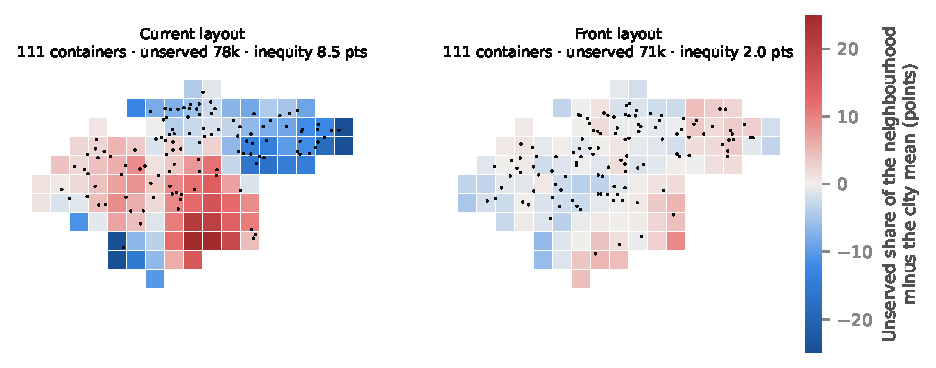
\includegraphics[width=0.95\textwidth]{figures/map_donostia.pdf}
    \caption{Donostia, 500\,m blocks colored by the unserved share of their 1\,km neighbourhood minus the city average, for the current layout (left) and the fairest layout with the same number of containers and no more unserved people, from the four-objective run with the median such fairness (right). Dots are the containers.}
    \label{fig:map}
\end{figure}

\subsection{Integration in a data space}
The method is deployed as a service of the CitCom.ai data space, which reads the inventory of containers of a city through NGSI-LD (Smart Data Models \texttt{WasteContainer} entities) from the city's connector, and the population from GHS-POP, so it can be applied to any city that publishes its containers. A job runs in a single low-priority process. With the recommended configuration (NSGA-II, four objectives, no crossover, 300 generations, 100 individuals), it computes the front of Valencia in under a minute on one core of the cluster, and in a few minutes in the deployed service, where it runs at low priority on a shared node with the 8,308 candidate sites of the city's data. The planner can then browse the front and display any of its layouts on a map, compared with the current one.
